% vim: set ai tw=80 fileencoding=utf8: 
%-------------------------------------------------------------------------------
\documentclass[
  % -- opções da classe memoir --
	12pt,				% tamanho da fonte
	openright,			% capítulos começam em pág ímpar (página vazia se preciso)
  %twoside,			% para impressão em verso e anverso. Oposto a oneside
  oneside,			% oposto de twoside, para nao gerar paginas 
	a4paper,			% tamanho do papel. 
	% -- opções da classe dc-uel --
	tcc,			% tipo do trabalho (opções: tcc, dissertacao, qualificacaoms)
	]{dc-uel}


% ---
% PACOTES
% ---

% ---
% Pacotes fundamentais 
% ---
\usepackage[T1]{fontenc}		% Selecao de codigos de fonte.
\usepackage[utf8]{inputenc}		% Codificacao do documento
\usepackage{graphicx}			% Inclusão de gráficos
% ---
		
% ---
% Pacotes adicionais, usados apenas no âmbito do Modelo Canônico do abnteX2
% ---
\usepackage{lipsum}				% para geração de dummy text
% ---

% ---
% Informações de dados para CAPA, FOLHA DE ROSTO e outros elementos
% ---
\titulo{Desenvolvimento de Técnicas de Paralelização de Código}
\tituloingles{Designing Techiniques for Code Paralellization}
\palavraschave{palavra chave1. palavra chave2.}
\palavraschaveingles{word 1. key word2.}
\autor{Luiz Guilherme Castilho Martins}
\citacaoautor{MARTINS, L. G. C.}
\data{2013}

\diadefesa{24 de novembro}
\orientador{Prof. Dr. Wesley Attrot} % É membro nato e presidente da Banca Examinadora
\membrobancadois{Prof. Dr. Segundo Membro da Banca}
\instmembrobancadois{Universidade Estadual de Londrina}
\membrobancatres{Prof. Msc. Terceiro Membro da Banca}
\instmembrobancatres{Universidade Estadual de Londrina}
% \membrobancaquatro{Prof. Esp. Quarto Membro da Banca}
% \instmembrobancaquatro{Universidade/Instituição do Quarto Membro da Banca}

% ---
% compila o indice
% ---
\makeindex
% ---

% ----
% Início do documento
% ----
\begin{document}

% Retira espaço extra obsoleto entre as frases.
\frenchspacing 

% ----------------------------------------------------------
% ELEMENTOS PRÉ-TEXTUAIS
% ----------------------------------------------------------
% \pretextual


%  % vim: set ai tw=80 fileencoding=utf8: 
%-------------------------------------------------------------------------------

\imprimircapa

%  % vim: set ai tw=80 fileencoding=utf8: 
%-------------------------------------------------------------------------------

\imprimirfolhaderosto*

\begin{fichacatalografica}
	\vspace*{\fill}					% Posição vertical
	\hrule							% Linha horizontal
	\begin{center}					% Minipage Centralizado
	\begin{minipage}[c]{12.5cm}		% Largura
	
	\imprimirautor
	
	\hspace{0.5cm} \imprimirtitulo  / \imprimirautor. --
	\imprimirlocal, \imprimirdata-
	
	\hspace{0.5cm} \pageref{LastPage} p. : il. (algumas color.) ; 30 cm.\\
	
	\hspace{0.5cm} \imprimirorientadorRotulo~\imprimirorientador\\
	
	\hspace{0.5cm}
	\parbox[t]{\textwidth}{\imprimirtipotrabalho~--~\imprimirinstituicao,
	\imprimirdata.}\\
	
	\hspace{0.5cm}
		1. Otimização.
		2. Tranformações-de-loops.
		I. Prof. Dr. Wesley Atrot.
		II\. Universidade Estadual de Londrina.\\
    %		IV\. Título\\ 			
	
	\hspace{8.75cm} CDU 02:141:005.7\\
	
	\end{minipage}
	\end{center}
	\hrule
\end{fichacatalografica}

%  % vim: set ai tw=80 fileencoding=utf8: 
%-------------------------------------------------------------------------------
\begin{errata}
Elemento opcional da% \citeonline[4.2.1.2]{NBR14724:2011}. Exemplo:

\vspace{\onelineskip}

FERRIGNO, C. R. A. \textbf{Tratamento de neoplasias ósseas apendiculares com
reimplantação de enxerto ósseo autólogo autoclavado associado ao plasma
rico em plaquetas}: estudo crítico na cirurgia de preservação de membro em
cães. 2011. 128 f. Tese (Livre-Docência) - Faculdade de Medicina Veterinária e
Zootecnia, Universidade de São Paulo, São Paulo, 2011.

\begin{table}[htb]
\center
\footnotesize
\begin{tabular}{|p{1.4cm}|p{1cm}|p{3cm}|p{3cm}|}
  \hline
   \textbf{Folha} & \textbf{Linha}  & \textbf{Onde se lê}  & \textbf{Leia-se}  \\
    \hline
    1 & 10 & auto-conclavo & autoconclavo\\
   \hline
\end{tabular}
\end{table}

\end{errata}

%  % vim: set ai tw=80 fileencoding=utf8: 
%-------------------------------------------------------------------------------

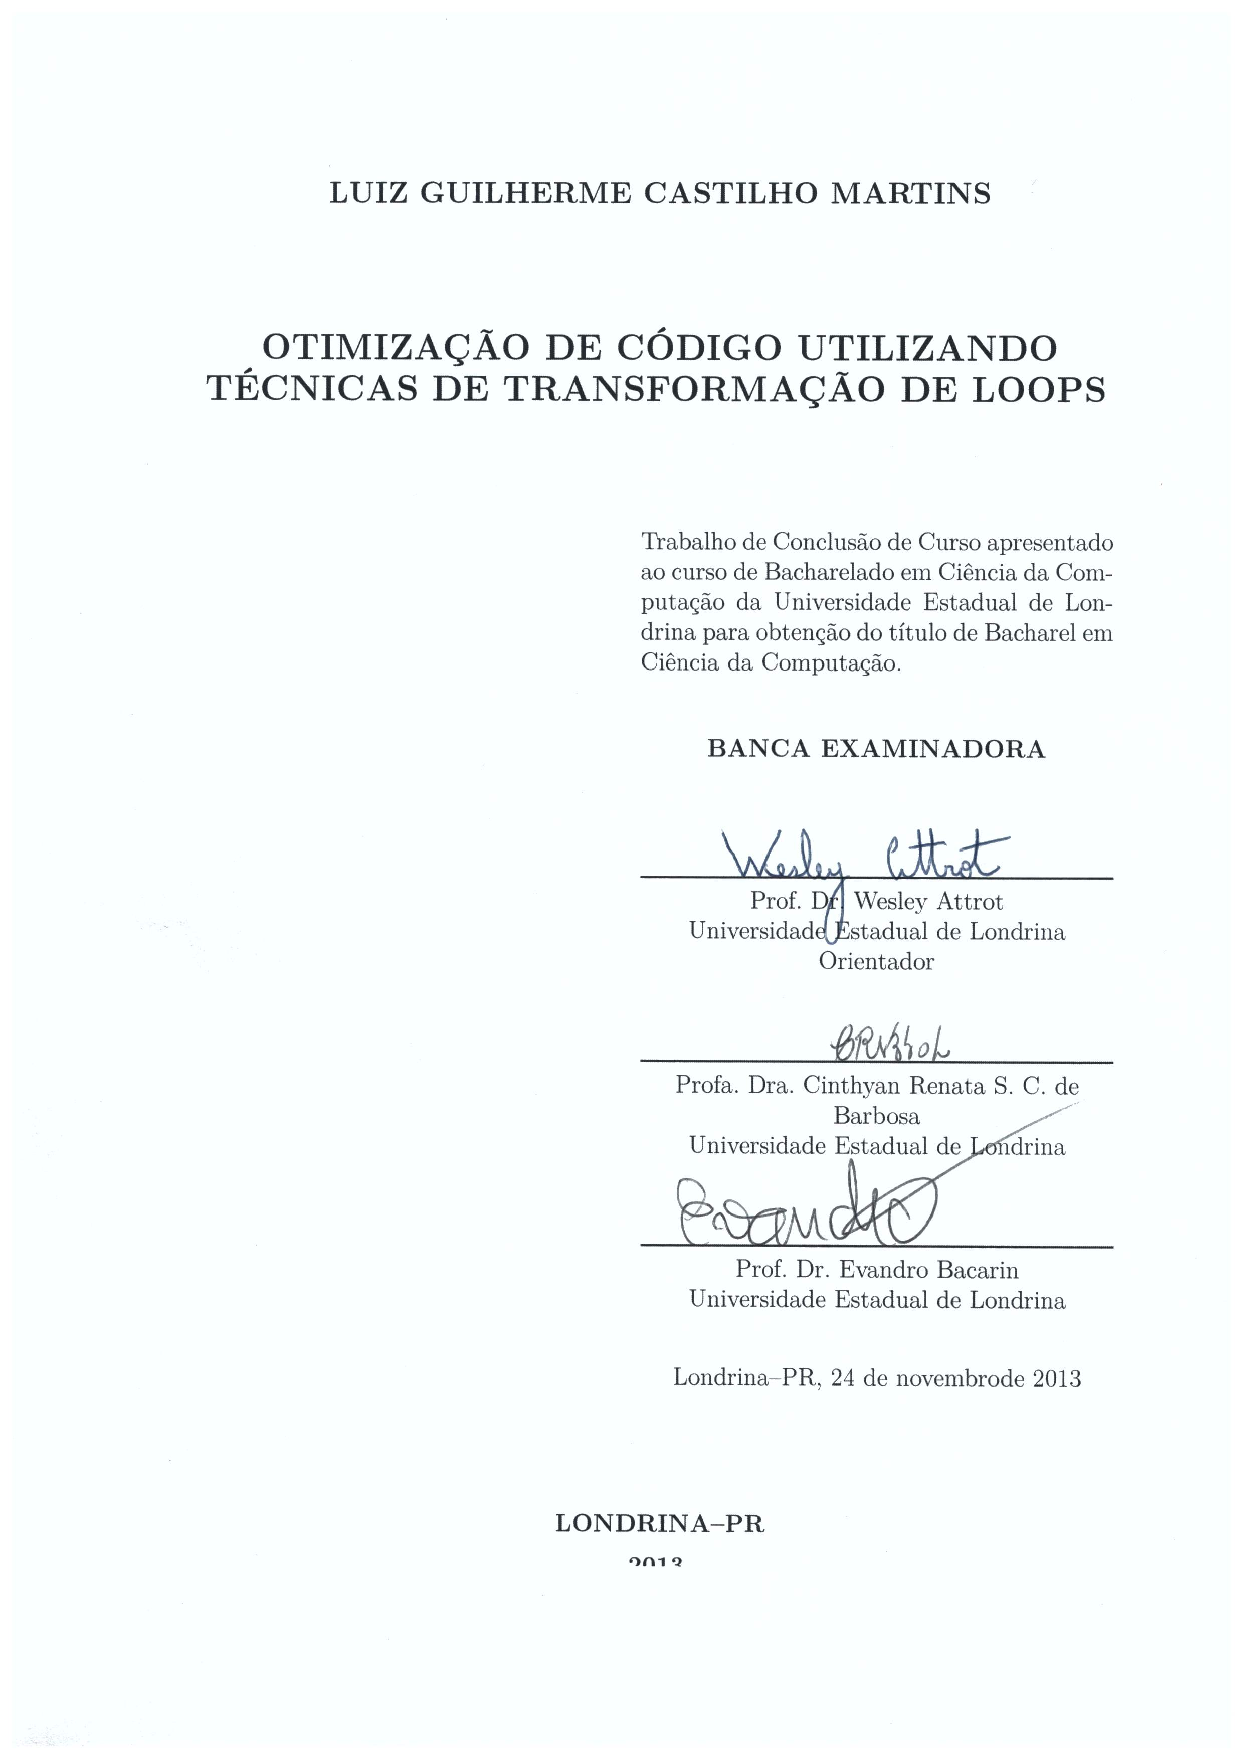
\includepdf{folha-aprovacao}

%  % vim: set ai tw=80 fileencoding=utf8: 
%-------------------------------------------------------------------------------
\begin{dedicatoria}
   \vspace*{\fill}
   \centering
   \noindent
	 \textit{A todos aqueles que \\ 
           me apoiaram e contribuíram \\ 
   para conclusão deste trabalho.} \vspace*{\fill}
\end{dedicatoria}


%  % vim: set ai tw=80 fileencoding=latin1: 
%-------------------------------------------------------------------------------

\newpage

\chapter*{AGRADECIMENTOS}

		\begin{trivlist}  \itemsep 2ex  \normalsize
					\item Agrade�o primeiramente aos meus pais por todo apoio que eles 
                me deram durante a gradua��o.
		\end{trivlist}

%  % vim: set ai tw=80 fileencoding=utf8: 
%-------------------------------------------------------------------------------
\begin{epigrafe}
    \vspace*{\fill}
	\begin{flushright}
		\textit{``O importante é ganhar. Tudo e sempre. \\
                Essa história que o importante é competir não passa de \\
                demagogia.\\
                (Ayrton Senna)}
	\end{flushright}
\end{epigrafe}

%  % vim: set ai tw=80 fileencoding=latin1: 
%-------------------------------------------------------------------------------

\newpage
\singlespacing
		\noindent MARTINS, Luiz Guilherme Castilho {\bf \titulotcc}. 2013. 
                173 f. TCC - Universidade Estadual de Londrina, 
                Londrina. 2013. \\
		\begin{center}
					{\bf {\Large RESUMO}}
		\end{center}

		\noindent Resumo.
    \newline

		\noindent{\bf Palavras-Chave:} palavra1, palavra2.

%  % vim: set ai tw=80 fileencoding=utf8: 
%-------------------------------------------------------------------------------
\begin{Abstract}
        The goal of this work is the optimization of computation of loops.
        Computationally expensive programs in general spend most of their time
        in the execution of loops.
        Loops with a large number of iterations over a big data arrays, those are
        the ones that spend of the process execution time.
        Thus, they are eligible to produce better results after optimization.
        Tecniques of loop transformation such as, loop unswitching, loop fission,
        loop fusion, loop unrolling, among others, was used in optimization.
        Analysis of data dependence was necessary to keep the meaning of the 
        program after the optimizations.
\end{Abstract}


%
%% ---
%% inserir lista de ilustrações
%% ---
%\pdfbookmark[0]{\listfigurename}{lof}
%\listoffigures*
%\cleardoublepage
%% ---
%
%% ---
%% inserir lista de tabelas
%% ---
%\pdfbookmark[0]{\listtablename}{lot}
%\listoftables*
%\cleardoublepage
%% ---
%
 % vim: set ai tw=80 fileencoding=utf8: 
%-------------------------------------------------------------------------------
\begin{siglas}
        % C
        \item[CPU] Central Processing Unit

        % D 
        \item [DFG] Data Flow Graph

        % I
        \item[IW] Instruction Word 

        % M
        \item[MISD] Multiple Instruction Single Data
        \item[MIMD] Multiple Instruction Multiple Data

        % N
        \item [NASA] National Aeronautics and Space Administration
        \item [NOWs] Network of Workstations

        % S
        \item[SISD] Single Instruction Single Data
        \item[SIMD] Single Instruction Multiple Data


        % V
        \item[VLIW] Very Long Instruction Word
\end{siglas}

%
%% vim: set ai tw=80 fileencoding=utf8: 
%-------------------------------------------------------------------------------
\begin{simbolos}
  \item[$ \delta $] Letra grega delta 
\end{simbolos}

%
%
% ---
% inserir o sumario
% ---
 \pdfbookmark[0]{\contentsname}{toc}
 \tableofcontents*
 \cleardoublepage
% ---
%
%\textual
%
%% vim: set ai tw=80 fileencoding=latin1: 
%-------------------------------------------------------------------------------
\chapter{INTRODU��O}

			%\noindent \begin{itemize}
			%			\item \indent Objetivos
			%			\item Objetivos secund�rios
			%			\item Fale sobre os objetivos do Brasil em se tornar independente tecnologicamente no desenvolvimento de microprocessadores.
			%\end{itemize}
\section{Motiva��o}
    \noindent texto.
    
\section{Objetivos e Contribui��es}

\section{Organiza��o do trabalho}

%
%% vim: set ai tw=80: 
%-------------------------------------------------------------------------------
\chapter{Taxonomia de Flynn}

\noindent Taxonomia de Flynn, proposta em 1966 \cite{Flynn:1966} por Michael 
Flynn e expandida em 1972 \cite{Flynn:1972}, � uma das formas de classificar o 
paralelismo dispon�vel no processador.  

Taxonomia de Flynn utiliza o conceito de sequ�ncia de objetos ou a��es, que s�o
chamados de \textit{stream}.
Flynn introduziu dois tipos de \textit{stream}, o 
\textit{stream} de instru��o e tamb�m o \textit{stream} de dados. 

O \textit{stream} de instru��o consiste em uma sequ�ncia de instru��es. 
Uma instru��o ou \textit{instruction word (IW)} � uma cadeia de 0's e 1's que 
representa a menor opera��o vis�vel ao programador e que ser� executada pelo 
processador. 
Uma instru��o pode conter uma ou mais opera��es, devido a isso
alguns autores utilizam \textit{instruction} para instru��es que contenham 
apenas uma opera��o e \textit{instruction word} para instru��es que contenham 
mais de uma opera��o.

\begin{comment}
Processadores escalares (\textit{scalar processors}) e processadores
superescalares (\textit{superscalar processors}) executam uma ou mais
\textit{instructions} por ciclo de \textit{clock} da m�quina. 
\end{comment}

Existem no entanto quatro combina��es de \textit{streams} que descrevem as 
arquiteturas de computadores mais comuns \cite{Flynn:1996}:

\begin{enumerate}
        \item \textbf{SISD:} \textit{Single Instruction, Single Data}
        \item \textbf{SIMD:} \textit{Single Instruction, Multiple Data}
        \item \textbf{MISD:} \textit{Multiple Instruction, Single Data}
        \item \textbf{MIMD:} \textit{Multiple Instruction, Multiple Data}
\end{enumerate}

Cada combina��o de \textit{stream} caracteriza uma classe de arquitetura 
e cada classe possui seus tipos de paralelismo.


%-------------------------------------------------------------------------------
\subsection{SISD: Single Instruction, Single Data}

\noindent A classe de arquiteturas de processadores \textit{SISD}, inclui a 
maior parte dos processadores utilizados nos dias de hoje, os processadores 
\textit{single-core}, embora os programadores n�o percebam o paralelismo 
inerente destes processadores, muita concorr�ncia pode estar presente.  

Em 1966 Flynn cita o \textit{Pipeline} como uma forma de se obter concorr�ncia 
nos processadores \textit{SISD}, embora ele considere a decodifica��o das 
in�meras \textit{instructions} como sendo um \textit{bottleneck}, devido a 
tecnologia da �poca. 
Nos dias de hoje, grande parte dos dos processadores 
utilizam-se de \textit{Pipeline} assim como tamb�m se aproveitam de alguma forma 
de m�ltiplas \textit{instructions}.

A concorr�ncia em processadores \textit{SISD} s�o explorados durante a execu��o,
realizando mais de uma opera��o por ciclo de \textit{clock} da m�quina.
%do \textit{stream} de instru��es.

A quantidade e o tipo de paralelismo poss�vel em processadores \textit{SISD}
� determinada por quatro fatores principais:

\begin{enumerate}
        \item O n�mero de opera��es que podem ser executadas concorrentemente.
        \item A forma como as opera��es ser�o arranjadas para execu��o,
                podendo ser estaticamente, dinamicamente ou at� mesmo das duas
                formas.
        \item A ordem em que as opera��es s�o colocadas e retiradas em rela��o
                a ordem original do programa.
        \item A maneira em o processador ir� tratar cada exce��o, podendo ser 
                preciso, impreciso ou das duas maneiras.
\end{enumerate}

%-------------------------------------------------------------------------------
\subsubsection{Processadores Escalares}

\noindent Processadores escalares s�o processadores simples, que executam no 
m�ximo uma instru��o e no m�ximo uma opera��o por ciclo de \textit{clock} de 
m�quina. 
As instru��es do \textit{stream} de instru��es s�o executadas 
sequencialmente, assim uma nova instru��o n�o ser� executada at� que a execu��o 
da instru��o em execu��o seja finalizada e seu resultado devidamente
armazenado.
A sem�ntica de instru��o determina que uma sequ�ncia de a��es devem ocorrer
para que se objenha o resultado esperado, sendo: buscar a instru��o,
decodifica-la, acessar o dado ou registrador, execu��o da opera��o e armazenar o
resultado. 
Podendo ocorrer \textit{overlap} entre as a��es mas o resultado deve
aparecer na ordem especificada.
Esse comportamento sequencial descreve o modelo de execu��o sequencial.
No modelo de execu��o sequencial, a execu��o � dita \textit{instruction-precise}
se encontrar as sequintes condi��es:

\begin{itemize}
        \item Todas as instru��es ou opera��es que precederam a instru��o atual
                ou opera��o atual j� foram executadas e seus resultados
                armazenados.
        \item Todas as instru��es ou opera��es na fila de execu��o n�o foram
                executadas ou seus resultados ainda n�o foram armazenados.
        \item A instru��o ou opera��o em execu��o no momento est� em um dos
                estados de execu��o, tendo ou n�o seu resultado j� armazenado.
\end{itemize}

A maioria dos processadores escalares implementam diretamente o modelo de
execu��o sequencial.


%-------------------------------------------------------------------------------
\subsubsection{Processadores Superescalares}

Enquando processadores escalares est�o limitados a executar uma �nica instru��o 
por ciclo de \textit{clock} de m�quina os processadores superescalares decoficam
v�rias instru��es por ciclo de \textit{clock} de m�quina, utilizando varios
unidades funcionais e aloca��o din�mica para executar v�rias instru��es por
ciclo de \textit{clock} de m�quina. 
Processadores superescalares tem um comportamente similar ao \textit{pipeline}.

A capacidade de executar m�ltiplas instru��es implica em verificar se existe
depend�ncias entre as instru��es, essa verifica��o tem que ser feita em n�vel de
\textit{hardware}. 
Processadores superescalares mais avan�ados geralmente incluem 
\textit{hardwares} que preservam a ordem e precisamente lida com as exce��es, 
assim simplificando o modelo de programa��o.

Devido a complexidade da l�gica para aloca��o din�mica das instru��es,
processadores superescalares de alto desempenho em geral est�o limitados a
executarem de quatro a oito instru��es por ciclo de \textit{clock} de m�quina.


%-------------------------------------------------------------------------------
\subsubsection{Processadores VLIW}

Processadores VLIW (\textit{Very Long Instruction Word}) assim como os
processadores superescalares decodificam in�meras instru��es por ciclo de
\textit{clock} de m�quina e utilizam v�rias unidades funcionais.

Ao contr�rio dos processadores superescalares que utilizam \textit{hardware}
para realizar aloca��o din�mica das instru��es os processadores VLIW executam as 
intru��es atrav�z de aloca��o est�tica, essa aloca��o depende de uma an�lise do
compilador.
Assim os processadores VLIW s�o menos complexos e apresentam desempenho 
potencialmente maior.

Para aplica��es que podem ser efetivamente alocada de forma est�tica os
processadores VLIW apresentam grande desempenho, embora nem todas as aplica��es
tenham esta caracterista assim a ordem de execu��o est�tica determinada pelo
compilador n�o seja procedente. 
Duas classes de execu��o podem ocorrer e afetar o comportamento da execu��o 
est�tica:

\begin{enumerate}
        \item Atrasos de resultados de opera��es devido a diferen�a da lat�ncia
                ocorrida com a lat�ncia considerada durante a aloca��o pelo
                compilador.
        \item Exce��es ou interrup��es que colocam a ordem de execu��o em um
                estado n�o antecipado pelo compilador.
\end{enumerate}

O processador consegue lidar com os atrasos, embora isso tenha um impacto 
significante no desempenho. 
A causa mais comum de atrasos na execu��o devem ao dado n�o estar mais na 
mem�ria cache, esse fator � tratado considerando-se o pior caso de lat�ncia 
poss�vel e at� evitando o uso da mem�ria cache. 
Na falta de paralelismo para cobrir as lacunas da lat�nica, resulta na 
aloca��o de instru��es com um n�mero menor de opera��es que o processador 
conseque executar, assim diminuindo o desempenho.


%-------------------------------------------------------------------------------
\subsection{SIMD: Single Instruction, Multiple Data}

\noindent A classe de processadores \textit{SIMD} incluem dois tipos de
processadores, vetoriais e matriciais.
Processadores \textit{SIMD} s�o projetados para utilizarem determinadas
estruturas de dados, como vetores e matrizes. 
Em n�vel de c�digo de m�quina, programar para processadores \textit{SIMD} � 
bastante similar a processadores \textit{SISD}, a diferen�a � realizar opera��es
nas estruturas de dados agregadas. Como no processamendo de algoritmos 
cient�ficos h� um grande uso de vetores e matrizes, processadores \textit{SIMD}
tem obtido grande desempenho na �rea.

Processadores vetoriais e matriciais apresentam diferen�as tando na 
implementa��o quando na organiza��o dos dados.

Processadores matriciais consistem em elementos de processos interconectados
cada um tendo seu pr�prio espa�o de mem�ria. Processadores vetoriais consistem
em um �nico processo que referencia a um espa�o de mem�ria global.

%-------------------------------------------------------------------------------
\subsubsection{Processadores Matriciais}


%-------------------------------------------------------------------------------
\subsubsection{Processadores Vetoriais}


%-------------------------------------------------------------------------------
\subsection{MISD: Multiple Instruction, Single Data}

\noindent A classe de processadores \textit{MISD} abstratamente � um
\textit{pipeline} de m�ltiplas unidades funcionais operando independentemente
sob um �nico \textit{stream} de dados. Em n�vel de micro-arquitetura �
exatamente o que os processadores vetoriais fazem.

Segundo \cite{Openshaw:1999} exceto no caso de um cientista da computa��o
interssado em estranhas formas de computa��o a classe \textit{MISD} � uma forma
restritiva e impratic�vel de paralelismo.

%-------------------------------------------------------------------------------
\subsection{MIMD: Multiple Instruction, Multiple Data}

\noindent Na classe de processadores \textit{MIMD} est�o os multiprocessadores
com alguma forma de interconex�o entre os processadores. Do ponto de vista do
programador, cada processo � executado independentemente e de forma cooperativa
para solucionar um mesmo problema, embora alguma forma de sincroniza��o entre os
processos � necess�ria para que as informa��es e dados sejam trocados entre os
processadores.

N�o existe limita��es em que todos os processadores sejam id�nticos, embora a
maioria das configura��es \textit{MIMD} s�o homog�nios, com processadores
id�nticos. Configura��es heterog�nias de processadores s�o geralmente utilizados
para aplica��es com prop�sitos esp�cificos.

Da perspectiva de \textit{hardware} exitem dois tipos de \textit{MIMD}, sendo os
processadores \textit{multi-cores} e processadores \textit{multi-threaded}.


%-------------------------------------------------------------------------------
\subsubsection{Processadores Multi-Threaded}


%-------------------------------------------------------------------------------
\subsubsection{Processadores Multi-Core}



%	
%% vim: set ai tw=80 fileencoding=utf8: 
%-------------------------------------------------------------------------------
\chapter{Memória}

A mais simples maneira de se melhorar o desempenho de um sistema é
replicar os computadores e criar uma forma destes trocarem dados.
Desta forma consegue-se aumentar o desempenho sem que seja necessário alterar a
\textit{CPU}.

Com o aumento contínuo da necessidade de desempenho em aplicações cada vez mais
custosas a maioria dos sistemas paralelos utilizam-se de uma entre duas
técnologias, memória distribuída ou memória compartilhada.


%-------------------------------------------------------------------------------
\section{Memória Distribuída}

Memória distribuída ou \textit{distributed memory} ou \textit{shared-nothing} é
a mais simples abordagem do ponto de vista do \textit{hardware}. 
A premissa desta abordagem é utilizar vários computadores interligados atravéz 
de uma rede.

O modelo padrão de programação consiste de processos separados para cada
computador que se comunicam atravéz da troca de mensagem ou 
\textit{message passing}, o que normalmente é feito atravéz de bibliotecas
desenvolvidas com esse propósito. 
Sendo este é o modelo mais clássico de computação paralela. 
A forma moderna de sistemas com memória distribuída iniciou a partir do trabalho 
de Seitz em 1985 \cite{Seitz:1985}.

Devido ao baixo custo de processadores voltados ao mercado consumidor e da fácil
montagem, alguns grupos exploraram tais fatores começaram a construir
\textit{cluster} de computadores pessoais. 
Tais \textit{clusters} já chamados de \textit{NOWs}, 
\textit{Network of Workstations}.
Combinando todos estes fatores com o rápido avanço de desempenho de computadores
pessoais e o avanço do \textit{open-source} junto com  versões de sistemas 
operacionais UNIX ajudaram a difundir sistemas com tais caracteristicas. 
Hoje estes sistemas são comumente conhecidos como \textit{Beowulfs} ou
\textit{Beowulf Cluster} devido ao projeto de Thomas Sterling e Donald Becker
realizado na NASA.

%-------------------------------------------------------------------------------
\section{Memória Compartilhada}

Memória compartilhada ou \textit{shared memory} é uma abordagem mais complexa, 
tornando a memória visível a todos os processadores, permitindo que 
todos possam carregar e gravar do mesmo endereço de memória. 

Entre as dificuldades desta abordagem os dois que chamam mais atenção são
coerência e consitência.
Sendo a consistência o mais problemático para o programador.




% ISA instruction set architecture

%referencias:
%sopc

%
 % vim: set ai tw=80 fileencoding=utf8: 
%-------------------------------------------------------------------------------

\chapter{Data Flow Graph}

\textit{Data Flow Graph} (DFG) ou grafo de fluxo de dados, é um modelo para 
programas que expressa a possibilidade de execução concorrênte de partes do
programa. 
Nos DFGs os nós representam operações (funções) e predicados a serem
aplicados a objetos de dados e as arestas representam a ligação entre o nó que
produz o dado ao nó que irá consumir aquele dado.
Na literatura os nós também são chamados de atores.
Assim, aspectos de controle e de dados de um programa podem ser representados 
em um único modelo integrado.

Embora muitas versões de DFGs tem sido estudadas na literatura, elas tem algumas
características em comum:

\begin{alineas}
        \item DFG é um grafo orientado onde uma aresta é um caminho que um dado
        percorre do nó produtor para o nó consumidor.
        \item Dinamicamente, o nó de um DFG aceita um ou mais dado como entrada,
        realizando computações e devolvendo os dados do retorno para suas
        saídas.
        \item Uma ação de um nó é ativada com a presença dos dados de entrada.
\end{alineas}

Os estudos em DFGs tem sido focado principalmente em três modelos bem definidos:
DFGs estáticos, DFGs dinâmicos e DFGs síncronos.

%eopc
%-------------------------------------------------------------------------------
%\section{Subcapítulo}




% ----------------------------------------------------------
% ELEMENTOS PÓS-TEXTUAIS
% ----------------------------------------------------------
\postextual


% ----------------------------------------------------------
% Referências bibliográficas
% ----------------------------------------------------------
\bibliography{3-taxonomia-flynn/taxonomia-flynn} 

\end{document}
